\documentclass[a4paper,11pt]{scrartcl}

\usepackage{graphicx}
\usepackage[utf8]{inputenc} 
\usepackage{amsmath,amssymb,amsthm} 
\usepackage[round]{natbib}
\usepackage{url}
\usepackage{xspace}
\usepackage[left=20mm,top=20mm]{geometry}
\usepackage{algorithmic}
\usepackage{subcaption}
\usepackage{mathpazo}
\usepackage{booktabs}
\usepackage{hyperref}
\hypersetup{
    colorlinks=true,
    linkcolor=black,
    filecolor=magenta,      
    urlcolor=cyan,
    citecolor=black,
}


\newcommand{\ie}{i.e.}
\newcommand{\eg}{e.g.}
\newcommand{\reffig}[1]{Figure~\ref{#1}}
\newcommand{\refsec}[1]{Section~\ref{#1}}

\setcapindent{1em} %-- for captions of Figures
\hbadness=10000 %-- set tolerance for under-full box
\hfuzz=10000pt %-- set tolerance for overfull box

\renewcommand{\algorithmicrequire}{\textbf{Input:}}
\renewcommand{\algorithmicensure}{\textbf{Output:}}


\title{PhD Thesis Proposal for Statistics track  \\  
    \large Hybrid Deep Learning Models for Financial Derivatives, 
Cryptocurrency and Investor Sentiment Analysis.}
\author{Odunayo Rotimi (\url{odun.rotimi@gmail.com}).}
\date{\today}


\begin{document}

\maketitle


%%%
%
\section{Rationale of research project}
Computational intelligence in finance has been an exceedingly popular topic for both academia and financial
industry in the last few decades. The dynamic nature of the finance discipline makes it a suitable field for
formulation, application, validation, and absorption of Machine Learning (ML) algorithms for financial
decision-making purposes. Stock market forecasting, algorithmic trading, credit risk assessment,
portfolio allocation, asset pricing and derivatives market are among the major areas where ML researchers
focused on, developing models that can provide working solutions to the financial sector's challenges.
\newline

That not withstanding, Deep Learning (DL) - a sub-field of ML - is gaining more traction in both the
literature and in application because of the accuracy it affords over traditional ML models. With growing
novelty in the design of DL algorithms, consisting in multiple Artificial Neural Network layers, these models provide high level
abstraction for data modelling. This ingenuity opens up a whole wide range of research opportunity that
could help advance the cause of the 4th industrial revolution in two dimensions. Firstly, relative to
transparency on the path of practitioners; and, secondly, to provide insights into the modelling techniques
for monitoring through policy formulations on the part of the regulatory bodies in the financial service sector.


%%%
%
\section{Problem identification}
In the literature the following is commonly observable:
\begin{enumerate}
    \item \label{pt-1} Most efforts geared towards DL research employ the use of hybrid models.This consists in the use problem-tailored model formulations that captures the intrinsic features of the relevant financial time series data. Studies have it that these models outperform the traditional forecasting models (\eg, see \citep{ozbayoglu2020deep}). Yet the literature on these innovative approach is scarce.
    \item \label{pt-2} The history of financial crisis has shown how, if financial industry and the their employed models are not properly regulated, can lead to a dwindling economy in a very short time. This is particularly more relevant for the industrial revolution, where majority of tasks and roles are computerized.
    \item \label{pt-3} In deference to \citep{sezer2020financial}, the commonly applied areas of predictive ML research include algorithmic trading, portfolio management and risk assessment. Definitive future-shaping areas such as cryptocurrency and block-chain technology is only beginning to enjoy little concrete research.
\end{enumerate}

Point (\ref{pt-1}) with respect to derivative pricing. Although there exist a wide-range of financial products serving the investment needs of investors and profitability objectives of service providers accordingly, survey has it that the financial derivative market seem not to have seen in-depth research relative to application of ML models in its pricing techniques. The argument in favor of this might not have far from the complexity required in pricing and modelling techniques and relatively short lifespan of most derivatives. That not withstanding, this area has been described as readily innovation absorbing in the literature.
\newline
On the other hand, it may be an argument in favor of the latter observation (i.e. (\ref{pt-3})) that cryptocurrency and block-chain may not have been assimilated into the industry-wide and/or world-wide usage as means of settlement of financial transactions. Granted, the acceptance will take a little while. However, research efforts in this domain not only serve the good of provision of ample opportunity of shaping the future of secure financial transactions; but also set formidable standards for a sustainable financial sector.
%%%
%
\section{Research aims and objectives}
\begin{enumerate}
    \item This thesis shall also inquire into the possibility of transforming financial information into information-flow graphs combined with Natural Language Processing techniques to study the inter-relatedness of investors' perception about trade information and how they drive resultant investment decisions. We shall then delve into predicting the inter-relatedness of the influence of trading news and possible dependence investment decisions on key sources or influencers using the emergent  Graph Convolutional Networks (GCN), designed to capture relational information. Performance will be  measured against that of other binary classification ML algorithms.
          Such transformation is well known in genetic modelling, communications and social networking. However, except for the experimental work of  \cite{weber2019anti} and application to stock trading (e.g. \cite{chen2018incorporating,wang2019alphastock}), there is but little known other instances where such transformation has been used in sentiment analysis. Such models, if carefully developed can help model investor behavior in automation-driven financial markets. \label{obj_1}
    \item The thesis aims to extend the novelty in developing mixed or hybrid Deep learning models that are viable for the prediction of derivatives. Method to be considered include the transformation of of financial data from 1-dimensional array to image-like 2-dimensional array in an effort to reduce associated dimensionality problems, combined with a parameterized version Neural Network (NN). Application of machine learning models to investment problems is well documented in the literature. \cite{ozbayoglu2020deep} is a rich resource for a comparative case study. The works of \cite{culkin2017machine, sezer2020financial} will constitute a starting point for transformation and model formulation respectively. \label{obj_2}
    \item Lastly, this research work extend the study of application of Generative Adversarial Network (GAN) to crypto-securities to contribute to the state of research. This aspect would detail a systematic enquiry comparative forecasting advantage the GAN may posses over other DL Models, building on the works of \cite{zola2020generative} and \cite{grilli2020generative}. \label{obj_3}
\end{enumerate}


%%%
%
\section{Research plan and methodology}
\subsection{Methodology}
The focus of this research shall be rather quantitative and theoretical in nature and would not require the use of questionnaire among practitioners.  The proposed models will be validated on financial time series trading data, derivative trading data as well as real-time news stream data where applicable. While the trading and derivatives data would be sourced from financial data terminals across Europe and American markets, I will also use \hyperlink{https://github.com/odunayo12/web-crawl}{data mining} (web scrapping) techniques to source other complementary data. This will facilitate the possibility of the use of relevant statistical metrics to evaluate our models. The limiting factor of this dissertation, however, would be that the proposed method methods need to be feasible for practical purposes: not only should it upscale when applied to sizable similar problems but also afford manageable computational time. The latter often constitute a topic of research on its own owing to the computational complexity and intensity of Machine Learning tasks.

%%%
%
% \subsection{Research plan}
% The project is proposed to last a 2 and half-year period, split into 4 phases (see \reffig{fig:my_label}). The first 6-month phase will center around review of the state of research and succeeded by another 6-month phase of data collection, analysis as well as validating of the existent ML models on the gathered data. This phase is targeted to culminate in a research paper worthy of publication in an internationally recognized research journal. Particularly, the third research objective is scheduled to have been fully addressed here.

% The third phase is scheduled to last one year. Here, time is intended to be invested in the bulk of theoretical model development, validation, and back-testing. Research objectives (\ref{obj_1}) and (\ref{obj_2}) shall be the focus of this stage. Deliverables include publication of research results in internationally recognized journal. The research will end with dissertation submission in phase 4.
% \begin{figure}[htb!]
%     \centering
%     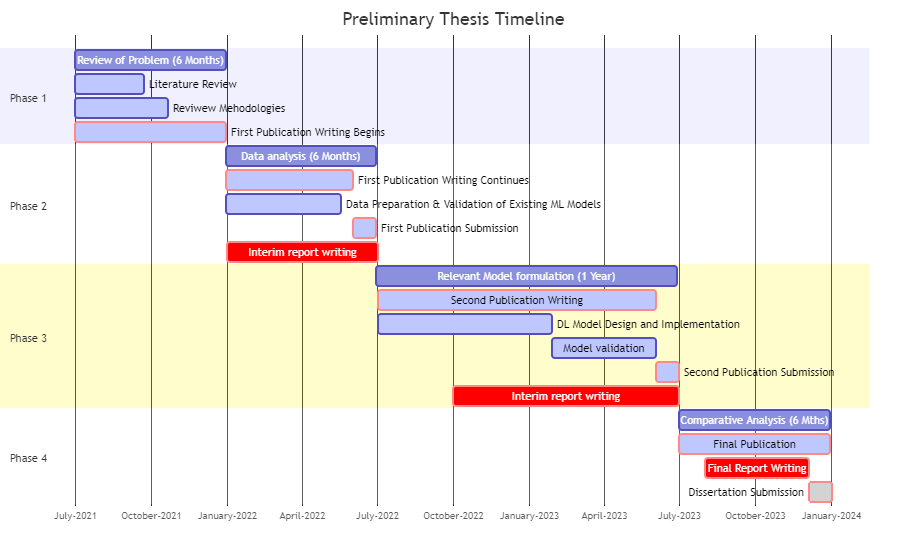
\includegraphics[width=\textwidth,height=8cm]{graphics/mermaid-diagram-2.png}
%     \caption{Timeline}
%     \label{fig:my_label}
% \end{figure}

\section{Expected research outputs}
The research findings and outcomes of this research work are proposed for publication in, but not limited to the following journals:
\begin{enumerate}
    \item Generative Adversarial Network (GAN) for Cryptocurrency | Journal of Statistical Software
    \item Hybrid Deep Learning Model for Financial Derivatives | Journal of Financial and Quantitative Analysis
    \item Graph Convolutional Networks (GCN) for Investor Sentiment Analysis | Applied and Computational Mathematics
\end{enumerate}

\bibliographystyle{abbrvnat}
\bibliography{myreferences}
\end{document}

